\documentclass[doc]{apa}
\usepackage[utopia]{mathdesign}
\usepackage{graphicx,apacite,amsmath,rotating,verbatim,epsfig,subfigure}
\usepackage{dcolumn}
\usepackage{tikz}

\title{mcplR: An R package to fit categorization and other multiple cue probability learning models}
\author{Maarten Speekenbrink}
\affiliation{Department of Psychology \\ University College London}

\abstract{

}

\ifapamodedoc{%
\leftheader{Speekenbrink}
\rightheader{MCPLR}
\acknowledgements{This research was supported by the ESRC Centre for Economic Learning and Social Evolution (ELSE).

Address correspondence to M. Speekenbrink, Department of Psychology, University College London, Gower Street, London WC1E 6BT, England, e-mail: \texttt{m.speekenbrink@ucl.ac.uk}}
}

\ifapamodejou{%
\leftheader{Speekenbrink}
\rightheader{MCPLR}
\acknowledgements{Address correspondence to M. Speekenbrink, Department of Psychology, University College London, Gower Street, London WC1E 6BT, England, e-mail: \texttt{m.speekenbrink@ucl.ac.uk}}
}

\ifapamodeman{%
	\note{
	\vspace{6em}
	\begin{flushleft}
    Dr. M. Speekenbrink\\
    Department of Psychology\\
    University College London \\
    Gower Street \\
    London WC1E 6BT \\ 
    England\\
    Tel:  +44 (0) 20 7679 7572 \\
    Fax: +44 (0) 20 7436 4276 \\
    E-mail: m.speekenbrink@ucl.ac.uk\\
   \end{flushleft}}}
{% else, i.e., in jou and doc mode 
\note{Draft of \today}}

\journal{To be submitted}

\renewcommand{\vec}[1]{\text{\bf{#1}}}
\newcommand{\mat}[1]{\text{\bf{#1}}}
\newcommand{\tr}{\text{tr}}
\newcommand{\logit}[1]{\log \left( \frac{#1}{1 - #1} \right)}
\newcommand{\logodds}[2]{\log \left( \frac{#1}{#2} \right)}
\newcommand{\slogit}[1]{\log( \tfrac{#1}{1 - #1})}
\newcommand{\mean}[1]{\overline{#1}}
\newcommand{\sign}{\text{sgn}}
\newcommand{\tif}{\text{ if }}

\newcommand{\greekv}[1]{\mbox{\boldmath$#1$}}
\newcommand{\greekm}[1]{\mbox{\boldmath$#1$}}
\newcommand{\thetab}{\mbox{\boldmath$\theta$}}
\newcommand{\betab}{\mbox{\boldmath$\beta$}}
\newcommand{\mub}{\mbox{\boldmath$\mu$}}
\newcommand{\Sigmab}{\mbox{\boldmath$\Sigma$}}
\newcommand{\sigmab}{\mbox{\boldmath$\sigma$}}
\newcommand{\MSE}{\text{MS}_e}
\newcommand{\diag}{\text{diag}}
\newcommand{\mtr}{^{\textsf{T}}}

\newcommand{\code}[1]{{\ttfamily{#1}}}
%\newcommand{\code}[1]{{\verb{#1}}}

\newcolumntype{d}[1]{D{.}{.}{#1}}

\begin{document}
\maketitle

Multiple Cue Probability Learning (MCPL) tasks require the prediction of a criterion variable on the basis of a number of cues which are probabilistically related to the criterion. This class of tasks is quite general, and a number of paradigms in (cognitive) psychology fall under it header. A numerical criterion variable is often used in Social Judgement Theory. When the criterion is a nominal variable, it is also common to speak of category learning tasks. 

A large number of formal models have been proposed to describe how people learn to perform MCPL tasks. We describe here an \code{R} package in which a number of these have been implemented, and which has been designed such that users can relatively easily add other models. 

We will describe the features of the package through the package's implementation of the Rescorla-Wagner. We will also briefly illustrate how to specify a new model. 

\section{The general structure of MCPL models}

In MCPL tasks, the objective is to predict a criterion variable $Y_t$ on the basis of a number of cues $X_{j,t}$. On each trial $t = 1,\ldots,T$, cue values are presented, and a prediction $R_t$ is made about the value of the criterion.

\begin{figure}
\centering
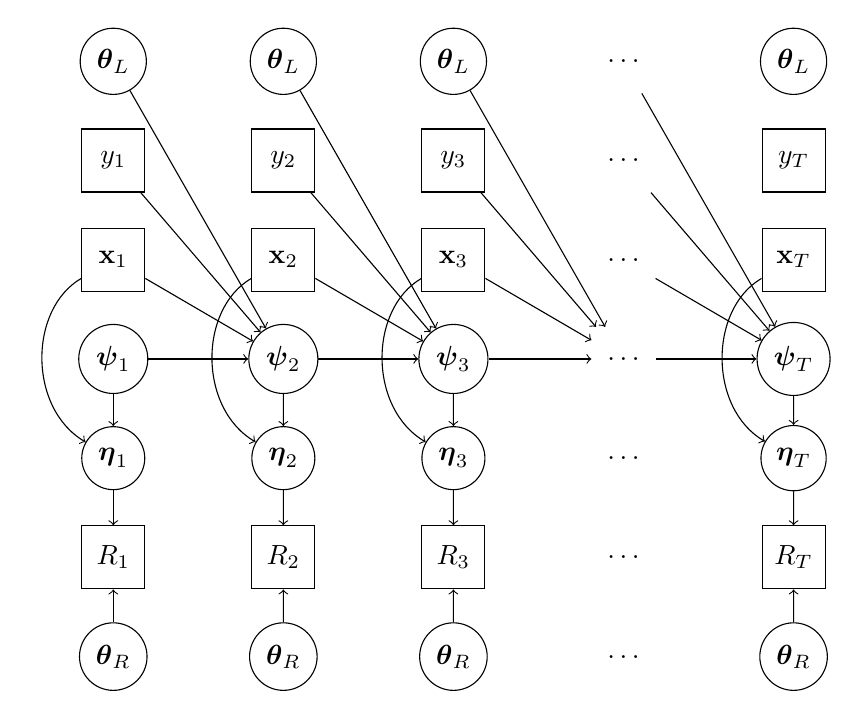
\begin{tikzpicture}[scale=.9]
		\begin{scope}[]{
			\pgfsetxvec{\pgfpoint{2.4cm}{0cm}}
			\pgfsetyvec{\pgfpoint{0cm}{1.4cm}}
			\tikzstyle{every node}=[minimum size=.8cm]


				\draw	node[draw,circle] (thetaR1) at (0,-2) {$\greekv{\theta}_R$};
				\draw node[draw,circle] (thetaR2) at (1,-2) {$\greekv{\theta}_R$};
			  \draw	node[draw,circle] (thetaR3) at (2,-2) {$\greekv{\theta}_R$};
				\draw	node (thetaRdots) at (3,-2) {$\ldots$};
				\draw	node[draw,circle] (thetaRT) at (4,-2)  {$\greekv{\theta}_R$};
				
				\draw	node[draw] (r1) at (0,-1) {$R_1$};
				\draw node[draw] (r2) at (1,-1) {$R_2$};
			  \draw	node[draw] (r3) at (2,-1) {$R_3$};
				\draw	node (rdots) at (3,-1) {$\ldots$};
				\draw	node[draw] (rT) at (4,-1)  {$R_T$};

				\draw	node[draw,circle] (eta1) at (0,0) {$\greekv{\eta}_1$};
				\draw node[draw,circle] (eta2) at (1,0) {$\greekv{\eta}_2$};
			  \draw	node[draw,circle] (eta3) at (2,0) {$\greekv{\eta}_3$};
				\draw	node (etadots) at (3,0) {$\ldots$};
				\draw	node[draw,circle] (etaT) at (4,0) {$\greekv{\eta}_T$};
								
				\draw node[circle,draw] (psi1) at (0,1) {${\greekv{\psi}}_1$};
				\draw node[circle,draw] (psi2) at (1,1) {${\greekv{\psi}}_2$};
				\draw	node[circle,draw] (psi3) at (2,1) {${\greekv{\psi}}_3$};
				\draw	node (psidots) at (3,1) {$\ldots$};
				\draw	node[circle,draw] (psiT) at (4,1) {${\greekv{\psi}}_T$};
							
				\draw node[draw] (x1) at (0,2) {$\vec{x}_1$};
				\draw node[draw] (x2) at (1,2) {$\vec{x}_2$};
				\draw	node[draw] (x3) at (2,2) {$\vec{x}_3$};
				\draw	node (xdots) at (3,2) {$\ldots$};
				\draw	node[draw] (xT) at (4,2) {$\vec{x}_T$};
				
				\draw node[draw] (y1) at (0,3) {$y_1$};
				\draw	node[draw] (y2) at (1,3) {$y_2$};
				\draw	node[draw] (y3) at (2,3) {$y_3$};
				\draw	node (ydots) at (3,3) {$\ldots$}; 
				\draw	node[draw] (yT) at (4,3) {$y_T$};

				\draw	node[draw,circle] (thetaL1) at (0,4) {$\greekv{\theta}_L$};
				\draw node[draw,circle] (thetaL2) at (1,4) {$\greekv{\theta}_L$};
			  \draw	node[draw,circle] (thetaL3) at (2,4) {$\greekv{\theta}_L$};
				\draw	node (thetaLdots) at (3,4) {$\ldots$};
				\draw	node[draw,circle] (thetaLT) at (4,4)  {$\greekv{\theta}_L$};
				
				\draw[->] (psi1) -- (eta1);
				\draw[->] (psi2) -- (eta2);
				\draw[->] (psi3) -- (eta3);
				\draw[->] (psiT) -- (etaT);
				
				\draw[->] (x1) .. controls (-.5,1.5) and (-.5,0.5) .. (eta1);
				\draw[->] (x2) .. controls (.5,1.5) and (.5,0.5) ..  (eta2);
				\draw[->] (x3) .. controls (1.5,1.5) and (1.5,0.5)  ..  (eta3);
				\draw[->] (xT) .. controls (3.5,1.5) and (3.5,0.5) ..  (etaT);
				
				\draw[->] (eta1) -- (r1);
				\draw[->] (eta2) -- (r2);
				\draw[->] (eta3) -- (r3);
				\draw[->] (etaT) -- (rT);				
				
				
				\draw[->] (thetaR1) -- (r1);
				\draw[->] (thetaR2) -- (r2);
				\draw[->] (thetaR3) -- (r3);
				\draw[->] (thetaRT) -- (rT);
				
				\draw[->] (psi1) -- (psi2);
				\draw[->] (psi2) -- (psi3);
				\draw[->] (psi3) -- (psidots);
				\draw[->] (psidots) -- (psiT);		
						
				\draw[->] (x1) -- (psi2);
				\draw[->] (x2) -- (psi3);
				\draw[->] (x3) -- (psidots);
				\draw[->] (xdots) -- (psiT);
							
				\draw[->] (y1) -- (psi2);
				\draw[->] (y2) -- (psi3);
				\draw[->] (y3) -- (psidots);
				\draw[->] (ydots) -- (psiT);
				
				\draw[->] (thetaL1) -- (psi2);
				\draw[->] (thetaL2) -- (psi3);
				\draw[->] (thetaL3) -- (psidots);
				\draw[->] (thetaLdots) -- (psiT);
				}
			\end{scope}

\end{tikzpicture}
\caption{Representation of an MCPL model. The learning model involves updating representations $\greekv{\psi}_{t+1}$ on the basis of $\vec{x}_t$ and $y_t$. Representations and cues are used to form a prediction $\greekv{\eta}_t$, which is the basis of responses $R_t$.}
\label{fig:mcplmodel}
\end{figure}

An MCPL model consists of a learning and response models. A learning model describes how a representation of the environment is updated as new data comes in. A response model describes how this representation is used to form predictions of the environment. A graphical representation is given in Figure~\ref{fig:mcplmodel}. A main feature of MCPL models is that responses $R_t$ are conditionally independent given representations $\psi_t$, i.e.
\begin{equation}
P(R_1,\ldots,R_T|\greekv{\eta}_1,\ldots,\greekv{\eta}_T,\greekv{\theta}_R) = \prod_{t=1}^T P(R_t|\greekv{\eta}_t,\greekv{\theta}_R)
\end{equation}
While the response model is always a statistical model, in many cases the learning model is not. In many learning models, representations are updated as
\begin{equation}
\greekv{\psi}_{t+1} = f(\greekv{\psi}_t,\vec{x}_t,y_t,\greekv{\theta}_L),
\end{equation}
where $f$ is some (non-linear) function. For instance, the Rescorla-Wagner model \cite{Rescorla72} involves updating stimulus response associations $\greekv{\psi}_t$ in this form. As we will see later, the GCM is different, but still deterministic, in the sense that a particular set of paired cue and criterion values $(\vec{x}_{1:t},y_{1:t})$ and parameters $\greekv{\theta}_L$ always result in the same representation $\greekv{\psi}_t$. There are exceptions to this (such as Anderson's \citeyear{Anderson91} Rational Model of Categorization), but these are currently not implemented in \code{mcplR}. Note that determinism is not a requirement to implement learning models in \code{mcplR}. However, the default estimation relies numerical optimization routines which will give inconsistent results if $\greekv{\psi}_{1:T}$ differs from iteration to iteration. Hence, for probabilistic learning models, a different estimation routine will have to be implemented.
 
\section{Implementation in \code{mcplR}}

MCPL models are implemented in \code{mcplR} through the \code{McplModel} class. The class has two slots: one for a \code{LearningModel} and one for a \code{ResponseModel}. Both these have a similar structure, and consist minimally of a (predictor) matrix $x$, a (criterion) matrix $y$, and a parameter list. For the learning model, the predictor matrix will usually contain the cues, and the criterion matrix the criterion. For the response model, the predictor matrix will usually contain $\greekv{\eta}$, and the response matrix the responses $R$. 

In the implementation of MCPL models, we distinguish between learning and response models. A learning model

At the heart of the mcplR package is the class \code{McplModel}. An \code{McplModel} contains of two submodels, namely a \code{LearningModel} and a \code{ResponseModel}. Both these are derived from a general \code{McplBaseModel}, which contains a slot for a dependent variable ($y$), a slot for predictor variables ($x$), and a slot for a list with parameters. For a \code{LearningModel}, the criterion will usually be the dependent variable, and the cues the predictor variables. For a \code{ResponseModel}, the dependent variable will usually be the response variable, and the predictor variables (some function of) the predictions of the learning model. Both learning and response model can contain free variables.

In addition to class definitions, the mcplR package defines a number of methods which operate on these classes. The most important from the users viewpoint is no doubt the \code{estimate} method, by which to obtain (ML) estimates of model parameters.  

Estimate:
\begin{enumerate}
\item Compute $\greekv{\psi}$ from $\vec{y}$ and $\vec{x}$. \code{fit(learningModel)}.
\item Compute $\greekv{\eta}$ from $\greekv{\psi}$ and $\vec{x}$. \code{responseModel@x <- predict(learningModel)} 
\end{enumerate}

\section{Example: the Rescorla-Wagner model}

The Rescorla-Wagner model of associative learning \cite{Rescorla72}.

From trial $t$ to $t+1$, the associative strength between a CS (cue) $j$ and US (criterion) $k$ is updated as
\begin{equation}
\psi_{j,k}(t+1) = \psi_{j,k}(t) + \alpha_j \beta_k(y_k(t)) (\lambda_k y_k(t) - \sum_i x_i(t) \psi_{i,k}(t)) .
\end{equation}
where $y_k(t)$ is the value of US $K$ at trial $t$ (this should be 0 when US $k$ is not present at $t$), $x_j(t)$ the value of the CS $j$ ate trial $t$ (again, this should be 0 when $j$ is not present at $t$), $\alpha_j$ the salience of CS $j$, and $\beta_k$ the rate parameter for US $k$, which can be dependent on the presence or absence of $y_k(t)$. 

\subsection{Creating a Rescorla-Wagner learning model}

A Rescorla-Wagner model can be created by calling \code{RescorlaWagner(formula,data,...)}. For instance, for an event $y$ with two levels, and four cues $x_j$, we can use 


\begin{figure}
\begin{verbatim}
# create a learning model
lMod <- RescorlaWagner(y ~ x1+x2+x3+x4,data=WPT,ntimes=c(200,200))
# create a response model
rMod <- RatioRuleResponse(r~1,data=WPT,ntimes=c(200,200))
# combine in an McplModel
mMod <- McplModel(lMod,rMod)
# estimate the free parameters
mMod <- estimate(mMod)
# summary
summary(mMod)
\end{verbatim}
\caption{Example code to create and estimate a Rescorla Wagner model} 
\end{figure}

\code{lMod <- RescorlaWagner(y \textasciitilde x1+x2+x3+x4,data=WPT)}

which will create a default Rescorla-Wagner model. We can view the default parameter values by calling \code{getPars(lMod)}.
 
\subsection{Creating an MCPL model}

\subsection{Estimating the model parameters}
 
\section{Other learning models currently implemented in \code{mcplR}}

\subsection{Single Layer Feedforward Network}

Associative learning models such as the Rescorla-Wagner model can be implemented by an artificial neural network \cite{Gluck88} with one input layer and one output layer. These networks are also known as Single Layer Feedforward Network models \cite<SLFN,>{Bishop95}.  

\subsection{Generalized Context Model}

GCM learning model can be created by the function \code{GCM(formula,data,...)}. This will create a default GCM model, with a city-block distance function and an exponential similarity gradient, with  The distance function can be changed to an euclidian or general Minkowski distance function by the option \code{distance=``euclidian''} or \code{distance=``minkowksi''}, respectively. An arbitrary function can also be used by using a function for the distance option. Similarly, the similarity gradient can be changed through the option \code{similarity=``gaussian''}. In addition, the version of the GCM allows the specification of a sampling function (or memory gradient). By default, this is set to uniform, but other options are a power and exponential function.
 
\subsection{ALCOVE}

ALCOVE \cite{Kruschke92}.



\bibliography{bibliography}



\end{document}

A GCM can be specified by the function \code{GCM(formula,data,parameters,...)}. This function creates an object of the class \code{GCM}, extending the \code{LearningModel} class. To estimate the model's parameters, we can call the \code{estimate(object,...)} method. This will result in estimates which maximize the likelihood of the criterion. However, we will often want to use the \code{GCM} model as part of an \code{McplModel}. The ``classical'' GCM \cite{Nosofsky86} uses
\begin{equation}
P(R=j) = \frac{S_j^\lambda}{\sum_{k=1}^K S_k^\lambda}
\end{equation}
which is implemented in \code{mcplR} by a \code{RatioRuleResponse} model. This can be created by calling \code{RatioRuleResponse(formula,...)}, where only the left-hand side of the \code{formula} is evaluated. Starting values for the parameters can be given by an optional \code{parameters} argument. If this argument is not given, default starting values will be used (in this case, $\lambda=1$).

\subsection{Learning Model}

The GCM is different from other learning models in that it does not involve . Rather, learning consists of storing exemplars $(\vec{x}_t,y_t)$. To keep within the present framework, we can take the representation $\greekv{\psi}_t(\vec{x})$ to be a function 

\subsection{Response Model}

The GCM assumes that responses follow Luce's ratio rule, such that
\begin{equation}
P(R = j|\vec{x}) = \frac{V_j^\lambda}{\sum_k V_k^\lambda}
\end{equation}
Note that that the value of $V_j$ is given by the learning model. The response model thus contains a single free parameter, $\lambda$.

\subsection{Estimation}

The freely estimable parameters of the GCM are collected in the parameter vector $\greekv{\theta} = (,\lambda)$. Maximum likelihood estimates of these parameters are obtained by numerical maximisation of the likelihood $P(R|\greekv{\theta})$, specified in the response model. By default, numerical optimization is done by the Nelder-Mead simplex algorithm as implemented in the \code{optim} function of \code{R}. Other estimation procedures can be specified at the level of specific classes deriving from \code{McplModel}. There is also a switch to allow conditional maximisation of the response model parameters. In some cases, maximum likelihood estimates of the response model parameters can be derived in closed form (conditional on the learning model parameters), so that conditional estimation can decrease the computation required.